\documentclass{article}

% options are:
% - abs: use absolute positioning for the picture
% - percent: use percent positioning for the picture (percent of longer dimension)
% - permil: ten times percent
\usepackage[abs]{overpic}

\usepackage{xcolor}

\begin{document}

\begin{figure}
  \centering
  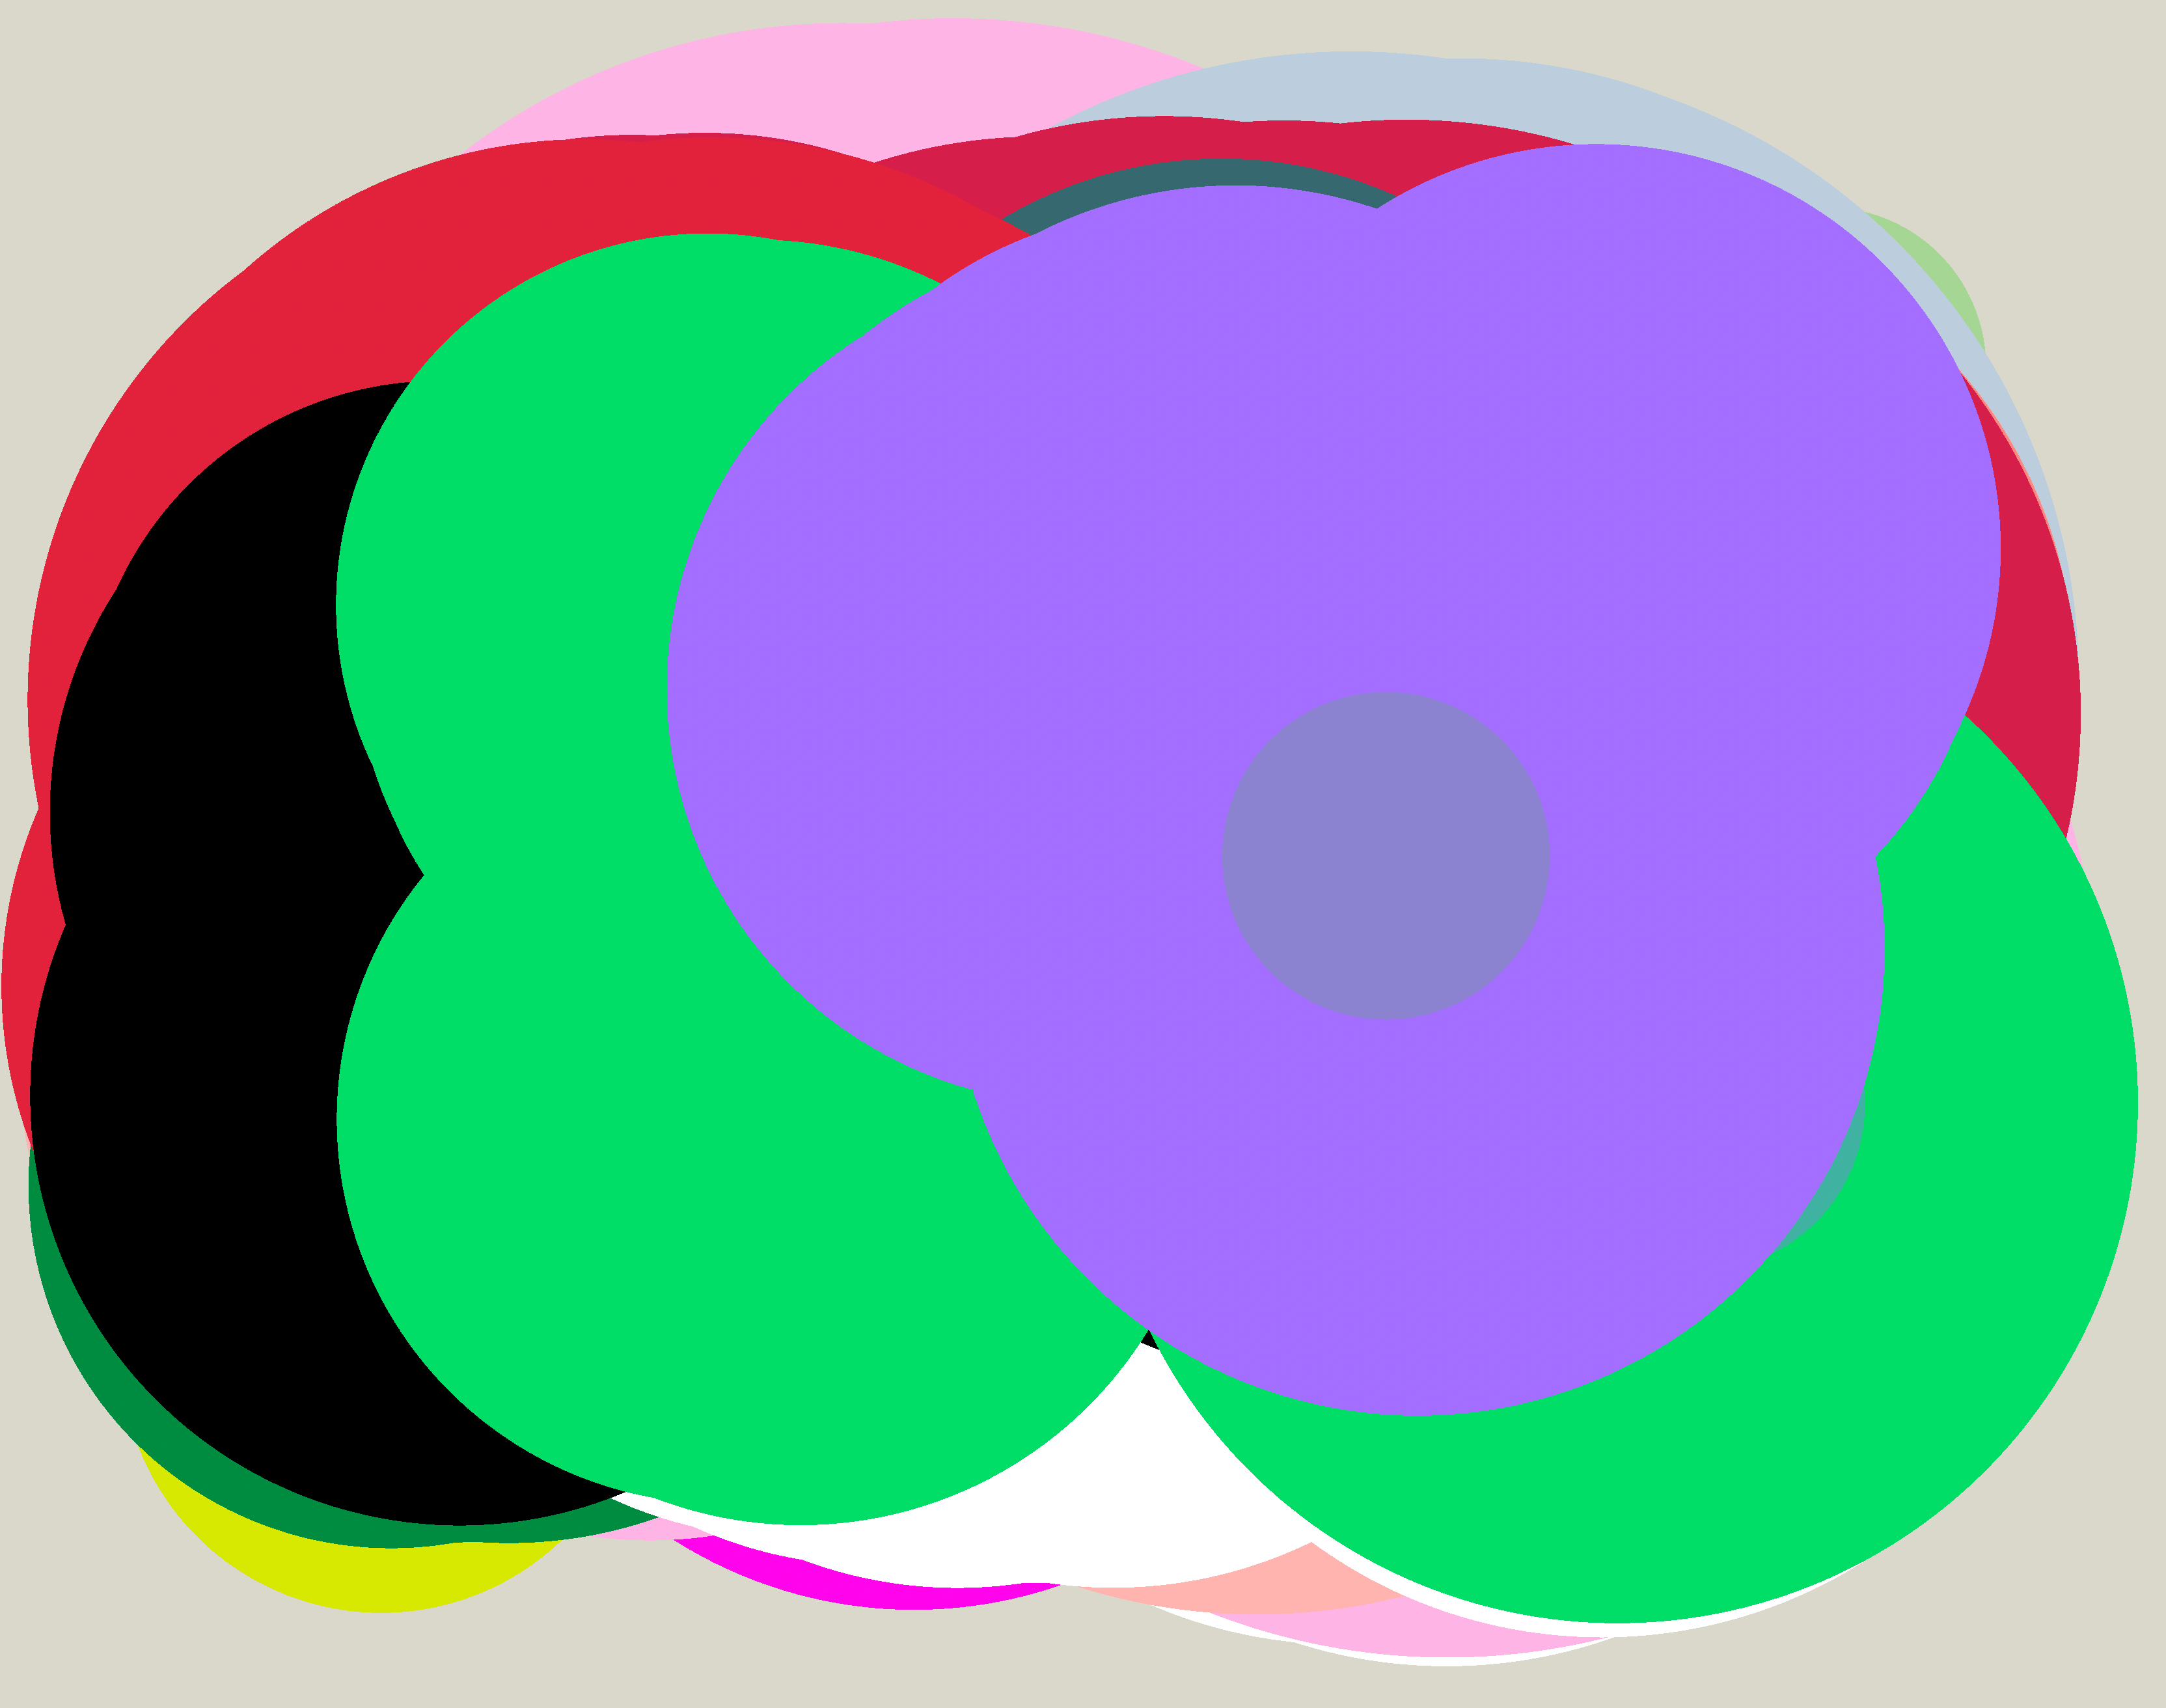
\includegraphics[width=0.8\columnwidth]{jack-circles.png}
  \label{fig:circles}
  \caption{Jack's wonderful circles, without text overlay}
\end{figure}

\begin{figure}
  \centering
  \begin{overpic}[width=0.8\columnwidth,grid,unit=1mm]{jack-circles.png}
    \put(2, 2){\textbf{(a)}}
    \put(60, 3){\Large\textbf{Jack Bentley}}
  \end{overpic}
  \label{fig:circles}
  \caption{Jack's wonderful circles, with text overlay, and a grid to help place text}
\end{figure}

\begin{figure}
  \centering
  \begin{overpic}[width=0.8\columnwidth,unit=1mm]{jack-circles.png}
    \put(2, 2){\textbf{(a)}}
    \put(60, 3){\Large\textbf{Jack Bentley}}
  \end{overpic}
  \label{fig:circles}
  \caption{Jack's wonderful circles, with text overlay, but without the grid}
\end{figure}

\end{document}
